%%%%%%%%%%%%%%%%%%%%%%%%%%%%%%%%%%%%%%%%%%%%%%%%%%%%%%%%%%%%
%%  This Beamer template was created by Cameron Bracken.
%%  Anyone can freely use or modify it for any purpose
%%  without attribution.
%%
%%  Last Modified: January 9, 2009
%%

\documentclass[xcolor=x11names,compress]{beamer}

%% General document %%%%%%%%%%%%%%%%%%%%%%%%%%%%%%%%%%
\usepackage{graphicx}
\usepackage{tikz}
\usepackage{amsmath}
\usepackage{amssymb}
\usepackage{amsthm}
\usepackage{acronym}
\usepackage{chngpage}
\usepackage{bbm}
\usepackage{tikz, overpic}
\usepackage{empheq} % autoloads mathtols and amsmath
\usepackage{multirow}%tex
\usepackage{pifont}
\usepackage{rotating}
\usepackage{subcaption}
\usepackage{pgfplots}
\usepackage{adjustbox}
\usetikzlibrary{decorations.fractals}

\newcommand{\bsum}[2]{\sum_{#1}^{#2}}
\newcommand{\bint}[2]{\int_{#1}^{#2}}
\newcommand{\E}[1]{\mathrm{E}(#1)}
\newcommand{\Var}[1]{\mathrm{Var}(#1)}
\newcommand{\Cov}[1]{\mathrm{Cov}(#1)}
\newcommand\given[1][]{\:#1\vert\:}
\newcommand{\for}{\;\text{for}\;}
\newcommand{\aand}{\;\text{and}\;}
\def\MLine#1{\par\hspace*{-\leftmargin}\parbox{\textwidth}{\[#1\]}}


%%%%%%%%%%%%%%%%%%%%%%%%%%%%%%%%%%%%%%%%%%%%%%%%%%%%%%


%% Beamer Layout %%%%%%%%%%%%%%%%%%%%%%%%%%%%%%%%%%
\useoutertheme[subsection=false,shadow]{miniframes}
\useinnertheme{default}
\usefonttheme{serif}
\usepackage{palatino}


\usetikzlibrary{bayesnet}


\setbeamerfont{title like}{shape=\scshape}
\setbeamerfont{frametitle}{shape=\scshape}

\setbeamercolor*{lower separation line head}{bg=DeepSkyBlue4} 
\setbeamercolor*{normal text}{fg=black,bg=white} 
\setbeamercolor*{alerted text}{fg=red} 
\setbeamercolor*{example text}{fg=black} 
\setbeamercolor*{structure}{fg=black} 
 
\setbeamercolor*{palette tertiary}{fg=black,bg=black!10} 
\setbeamercolor*{palette quaternary}{fg=black,bg=black!10} 

\addtobeamertemplate{navigation symbols}{}{%
    \usebeamerfont{footline}%
    \usebeamercolor[fg]{footline}%
    \hspace{1em}%
    \insertframenumber/\inserttotalframenumber
}


\renewcommand{\(}{\begin{columns}}
\renewcommand{\)}{\end{columns}}
\newcommand{\<}[1]{\begin{column}{#1}}
\renewcommand{\>}{\end{column}}
%%%%%%%%%%%%%%%%%%%%%%%%%%%%%%%%%%%%%%%%%%%%%%%%%%




\begin{document}

\pgfmathdeclarefunction{gauss}{2}{%
  \pgfmathparse{1/(#2*sqrt(2*pi))*exp(-((x-#1)^2)/(2*#2^2))}%
}
\pgfmathdeclarefunction{line}{1}{%
  \pgfmathparse{#1}%
}



%%%%%%%%%%%%%%%%%%%%%%%%%%%%%%%%%%%%%%%%%%%%%%%%%%%%%%
%%%%%%%%%%%%%%%%%%%%%%%%%%%%%%%%%%%%%%%%%%%%%%%%%%%%%%
\section{\scshape Supplmental}
\subsection{Original Model Selection}
\begin{frame}{Model Selection}
\onslide<1->{
\begin{table}[H] \centering 
\begin{tabular}{@{\extracolsep{5pt}} ccccc} 
\\[-1.8ex]\hline 
\hline \\[-1.8ex] 
Selection Based On &  $\mu$ &  $\sigma$ &  $\beta$ &  $\tau$ \\ \hline
\hline \\[-1.8ex] 
Brier Score & $35$ & $9$ & $8$ & $0.400$ \\ 
Error Rate & $35$ & $7.500$ & $19.500$ & $0.700$ \\ 
\hline \\[-1.8ex] 
\end{tabular} 
\caption{Na\"{i}ve Match Level Model Selection}
\end{table} 
}
\onslide<2>{
\vspace{-0.5cm}
\begin{table}[H] \centering 
\begin{tabular}{@{\extracolsep{5pt}} ccccc} 
\\[-1.8ex]\hline 
\hline \\[-1.8ex] 
Selection Based On &  $\mu$ &  $\sigma$ &  $\beta$ &  $\tau$ \\ \hline
\hline \\[-1.8ex] 
Brier Score & $35$ & $8$ & $21$ & $0.020$ \\ 
Error Rate & $35$ & $8$ & $18$ & $0.020$ \\ 
\hline \\[-1.8ex] 
\end{tabular} 
\caption{Na\"{i}ve Point Level Model Selection}
\end{table} 
}

\end{frame}

\subsection{Graphs}


\begin{frame}{Cross-Validation Graphs}
	\onslide<1>{
	\begin{figure}
		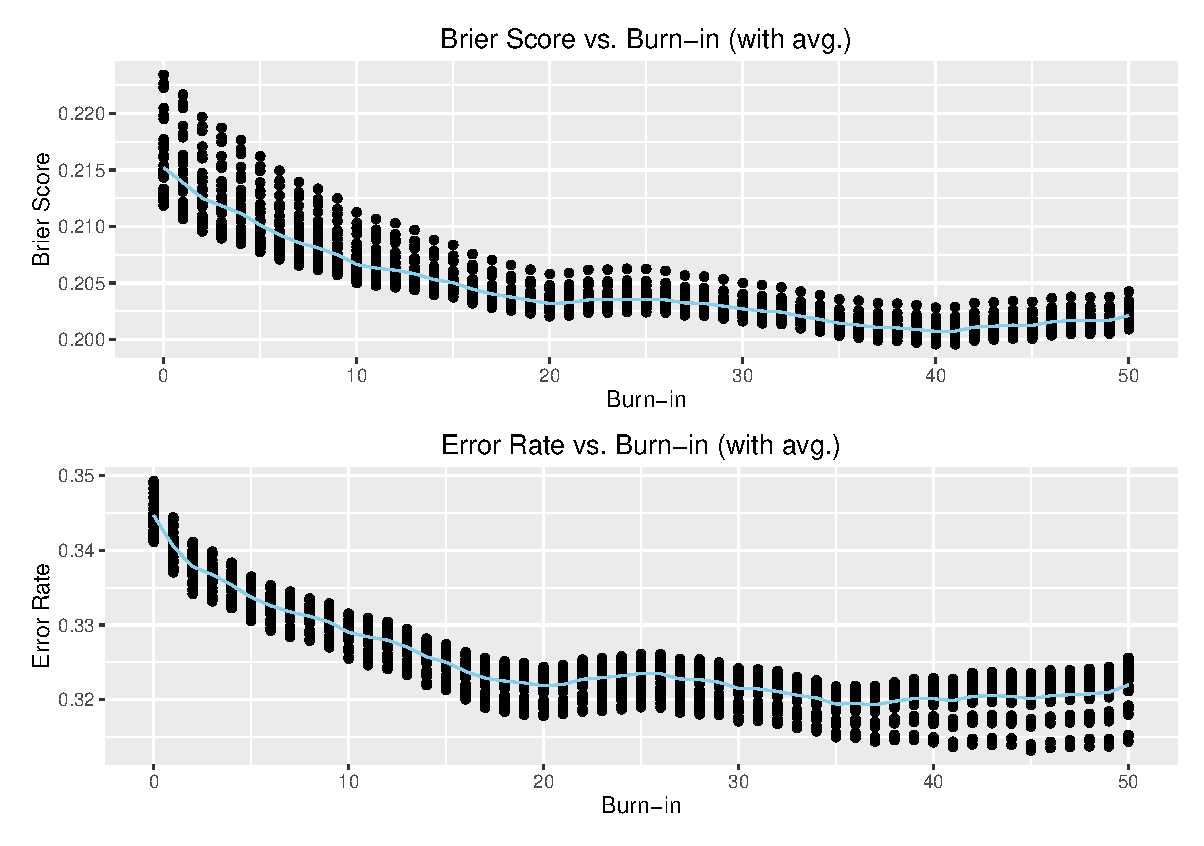
\includegraphics[width=0.95\linewidth]{figures/he.eps}
		\vspace{-0.1cm}
		\caption{Match Level Brier Score/Error Rate Verus Burn-In}
	\end{figure}}
	
\end{frame}


% approx here
\begin{frame}{Approximate Message Passing}

\begin{columns}
	\begin{column}{0.33\textwidth}
			\begin{tikzpicture}[scale=0.33]
\begin{axis}[ymin=0,ymax=2,xmax=3,xmin=-3,xticklabel=\empty,yticklabel=\empty,
               minor tick num=1,axis lines = middle,xlabel=$x$,ylabel=$y$,label style =
               {at={(ticklabel cs:1.1)}},samples=100]
	\addplot [very thick,cyan!50!black] {gauss(0,0.25)};
\end{axis}


\end{tikzpicture}
\onslide<3->{

\begin{tikzpicture}[scale=0.33]
\begin{axis}[ymin=0,ymax=2,xmax=3,xmin=-3,xticklabel=\empty,yticklabel=\empty,
               minor tick num=1,axis lines = middle,xlabel=$x$,ylabel=$y$,label style =
               {at={(ticklabel cs:1.1)}},samples=100]
	\addplot [very thick,cyan!50!black] {gauss(0,0.25)};
\end{axis}


\end{tikzpicture}
}
	\end{column}
	\begin{column}{0.33\textwidth}
			\begin{tikzpicture}[scale=0.33]
\begin{axis}[ymin=0,ymax=1.84,xmax=3,xmin=-3,xticklabel=\empty,yticklabel=\empty,
               minor tick num=1,axis lines = middle,xlabel=$x$,ylabel=$y$,label style =
               {at={(ticklabel cs:1.1)}},samples=100]
	\addplot [very thick,cyan!50!black, domain=-5:0] {line(0)};
	\addplot [very thick,cyan!50!black, domain=0:5] {line(1)};
\end{axis}

\end{tikzpicture}
\onslide<4->{
\begin{tikzpicture}[scale=0.33]
\begin{axis}[ymin=0,ymax=2,xmax=3,xmin=-3,xticklabel=\empty,yticklabel=\empty,
               minor tick num=1,axis lines = middle,xlabel=$x$,ylabel=$y$,label style =
               {at={(ticklabel cs:1.1)}},samples=100]
	\addplot [very thick,cyan!50!black] {gauss(0.6205,0.14)};
\end{axis}

\end{tikzpicture}
}
	\end{column}
	\begin{column}{0.33\textwidth}
			\begin{tikzpicture}[scale=0.33]
\begin{axis}[ymin=0,ymax=2,xmax=3,xmin=-3,xticklabel=\empty,yticklabel=\empty,
               minor tick num=1,axis lines = middle,xlabel=$x$,ylabel=$y$,label style =
               {at={(ticklabel cs:1.1)}},samples=100]
	\addplot [very thick,cyan!50!black, domain=0:5] {gauss(0,0.25)};
	\addplot [very thick,cyan!50!black, domain=-5:0] {line(0)};
	
\end{axis}

\end{tikzpicture}
\onslide<2->{
\begin{tikzpicture}[scale=0.33]
\begin{axis}[ymin=0,ymax=2,xmax=3,xmin=-3,xticklabel=\empty,yticklabel=\empty,
               minor tick num=1,axis lines = middle,xlabel=$x$,ylabel=$y$,label style =
               {at={(ticklabel cs:1.1)}},samples=100]
	\addplot [very thick,cyan!50!black, domain=0:5] {gauss(0.3989,0.090845)};
	
\end{axis}

\end{tikzpicture}
}
	\end{column}
\end{columns}
\end{frame}


\begin{frame}{Extension Attempt $1$}
\begin{adjustbox}{max totalsize={1\textwidth}{.9\textheight},center}
    \begin{tikzpicture}[scale=0.33]
        % left
        \factor[]{s-factor1}{above:$\mathcal{N}(s_1 \given \mu_1, \sigma_1^2+\tau^2)$}{}{};
        \node[latent, below=of s-factor1, yshift=0.5cm] (s1) {$s_1$};
        \factor[below=of s1, yshift=-0.5cm]{sp-factor1}{left:$\mathcal{N}(p_1 \given s_1 + \delta_s(st_1) , \beta^2 + \delta_b(st_1))$} {}{};
        \node[latent, below=of sp-factor1, yshift=0.5cm] (p1) {$p_1$};
        \factor[below=of p1] {pt-factor1} {left:$\mathbbm{I}(t_1=p_1)$}{}{};
        \node[latent, below=of pt-factor1, yshift=0.5cm] (t1) {$t_1$};
        
        % left-connections
        \edge[-]{s-factor1}{s1}
        \edge[-]{s1}{sp-factor1}
        \edge[-]{sp-factor1}{p1}
        \edge[-]{p1}{pt-factor1}
        \edge[-]{pt-factor1}{t1}
        
        
        % right
        \factor[right=of s-factor1,xshift=3cm]{s-factor2}{above:$\mathcal{N}(s_2 \given \mu_2, \sigma_2^2+\tau^2)$}{}{};
        \node[latent, below=of s-factor2, yshift=0.5cm] (s2) {$s_2$};
        \factor[below=of s2, yshift=-0.5cm]{sp-factor2}{right:$\mathcal{N}(p_2 \given s_2 + \delta_s(st_2), \beta^2 + \delta_b(st_2))$} {}{};
        \node[latent, below=of sp-factor2, yshift=0.5cm] (p2) {$p_2$};
        \factor[below=of p2] {pt-factor2} {left:$\mathbbm{I}(t_2=p_2)$}{}{};
        \node[latent, below=of pt-factor2, yshift=0.5cm] (t2) {$t_2$};
        
        % right-connections
        \edge[-]{s-factor2}{s2}
        \edge[-]{s2}{sp-factor2}
        \edge[-]{sp-factor2}{p2}
        \edge[-]{p2}{pt-factor2}
        \edge[-]{pt-factor2}{t2}
        
        % middle 
        \factor[below=of t1, xshift=2cm, yshift=-0.5cm] {td-factor} {left:$\mathbbm{I}(d=t_1-t_2)$}{}{};
        \node[latent, below=of td-factor](d) {$d$};
        \factor[below=of d, yshift=-0.5cm] {d-factor} {left:$\mathbbm{I}(d>\epsilon)$}{}{};
        
        % middle-connections
        \edge[-]{t1}{td-factor}
        \edge[-]{t2}{td-factor}
        \edge[-]{td-factor}{d}
        \edge[-]{d}{d-factor}
        
        
        \end{tikzpicture}
\end{adjustbox}
\end{frame}


\subsection{Synthetic Dataset Experiment}
\begin{frame}{Result On Synthetic Dataset}
	\onslide<1>{
	\begin{figure}
		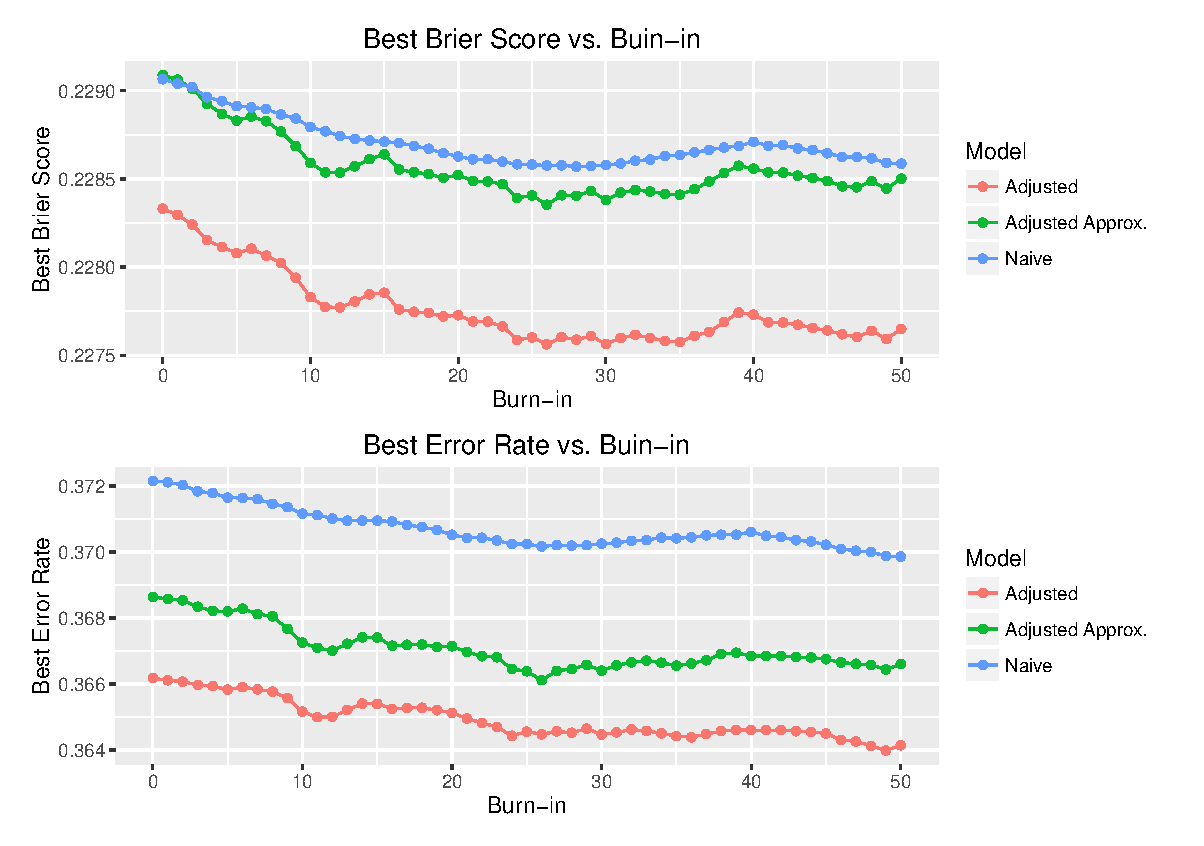
\includegraphics[width=0.95\linewidth]{figures/adjust.eps}
	\end{figure}}
\end{frame}

\begin{frame}{Results On ATP Dataset}

\begin{table}[H] \centering 
\begin{tabular}{@{\extracolsep{5pt}} ccccccc} 
\\[-1.8ex]\hline 
\hline \\[-1.8ex] 
$\mu$ &  $\sigma$ &  $\beta$ &  $\tau$ & $\mu_{\text{adj}}$ & $\sigma_{\text{adj}}$ & $\tau_{\text{adj}}$ \\ \hline
\hline \\[-1.8ex] 
$35$ & $8$ & $10$ & $0.020$ & $0$ & $2$ & $0.02$ \\ 
\hline \\[-1.8ex] 
\end{tabular} 
\caption{State-Aware Point Level Model Selection}
\end{table} 





\end{frame}









\end{document}
